%\documentclass[preprint]{aastex}  % USE THIS TO MAKE BIB, THEN FORMAT USING EMULATEAPJ
\documentclass[twocolumn,numberedappendix]{emulateapj}
\shorttitle{PSA64}
\shortauthors{Parsons, et al.}

\usepackage{amsmath}
\usepackage{graphicx}
\usepackage[figuresright]{rotating}
%\usepackage{rotating}
\usepackage{natbib}
%\usepackage{pdflscape}
%\usepackage{lscape}
\citestyle{aa}

\def\b{\mathbf{b}}
\def\k{\mathbf{k}}
\def\r{\mathbf{r}}
\def\q{\mathbf{q}}
\def\b{\mathbf{b}}
\def\kp{\mathbf{k}^\prime}
\def\kpp{\mathbf{k}^{\prime\prime}}
\def\V{\mathbb{V}}
\def\At{\tilde{A}}
\def\Vt{\tilde{V}}
\def\Tt{\tilde{T}}
\def\tb{\langle T_b\rangle}
\newcommand{\vis}{\mathbf{v}}
\newcommand{\x}{\mathbf{x}}
\newcommand{\xhat}{\hat{\mathbf{x}}}
\newcommand{\A}{\mathbf{A}}
\newcommand{\N}{\mathbf{N}}
\newcommand{\rhat}{\hat{\mathbf{r}}}

\begin{document}
\title{PSA-64 Power Spectrum}

\author{
Zaki S. Ali\altaffilmark{1},
Aaron R. Parsons\altaffilmark{1,2},
Adrian Liu\altaffilmark{1},
James E. Aguirre\altaffilmark{3},
David R. DeBoer\altaffilmark{2},
Daniel C. Jacobs\altaffilmark{8},
David F. Moore\altaffilmark{3},
Jonathan C. Pober\altaffilmark{4},
Jeff Zheng
% XXX if includes paper data, needs full author list
}

\altaffiltext{1}{Astronomy Dept., U. California, Berkeley, CA}
\altaffiltext{2}{Radio Astronomy Lab., U. California, Berkeley, CA}
\altaffiltext{3}{Dept. of Physics and Astronomy, U. Pennsylvania, Philadelphia, PA}
\altaffiltext{4}{Physics Dept.  U. Washington, Seattle, WA}
\altaffiltext{8}{School of Earth and Space Exploration, Arizona State U., Tempe, AZ}

\begin{abstract}
\end{abstract}

% XXX fringe weighting profile
% XXX delay spectrum not violated by freq-dependent fringe rate weights

\section{Introduction}
The Donald C. Backer Precision Array for Probing the Epoch of Reionization
(PAPER) is a dedicated experiment to measure the power spectrum of highly
redshifted 21 cm emission from the Epoch of Reionization.





\section{Observations}
Here, we describe the features of the data set used in this analysis. 
We used the maximally redundant configuration of the PAPER array (see Figure
\ref{fig:antenna_positions} for this analysis, relying on all of the redundant
baselines for the calibration procedure, but only using a subset of the
baselines for the power spectrum analysis. For the power spectrum analysis we
are using the baselines that correspond to the width between two columns (e.g.
49-41) as well as those that correspond to over and up and down one antenna
(e.g. 10-41 and 10-58, respectively). These 154 baselines are used in the power
spectrum analysis because they are instantaneously redundant and therefore they
measure the same Fourier modes on the sky. The sensitivity of the array is mostly
captured by these baselines. 

The observation of the 64 antenna data set spanned a 135 day period that
commenced on 2012 November 8 (JD62456240) and ended  2013 March 23 (JD62456375). 
Each baseline instantaneously measured the 100-200 MHz band which was divided
into 1024 frequency channels of resolution 97.66 kHz and integrated for 10.7
seconds.  

\subsection{Compressing the Data}
The raw described above constitue XX TB of data which can be cumbersome and time
consuming to do meaningful science. Therefore, the raw data was reprocessed
through a compression algorithm that comprised of chopping bits of data out that
correspondend to parts of the sky that was not relavant to our science
objectives. By applying fourier filters in the delay (Fourier dual of frequency)
and fringe rate (Fourier dual of time) spaces, we are able disregard 

\begin{figure*}\centering
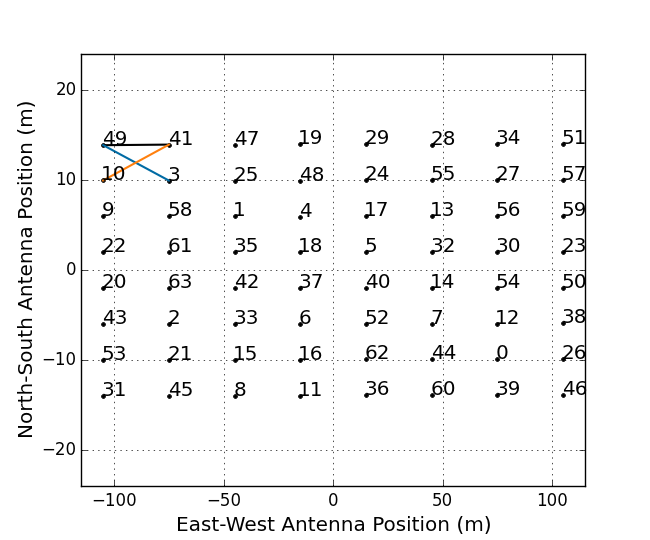
\includegraphics[width=1.85\columnwidth]{plots/antenna_positions.png}
\caption{Antenna positions for the PAPER 64 observation run.}
\label{fig:antenna_positions}
\end{figure*}

\section{Summary of Improvements from PSA32}
In comparison to the previous PAPER pipeline (see Parsonsi, 2014), this analysis
took a slightly different approach which included some important steps to
improve our bottom line. In short, the improvements included using a new, 
refined redundant calibration method (Zheng 2014), increasing the width of the
wideband delay filter that removes smothe spectrum foregrounds, weighting the
lst binned data sets, and optimal fringe rate filtering. 

Figure \ref{fig:step_through_pspec} shows the power spectra when each of the
steps mentioned above are turned off and for the one where all of them are
turned on.


%A more rigorous calibrations. Forward Ref.
%omnical
%lstbinning with chi-sq weighting
%horizon cut at 200ns = 100 + 100 (instead of 100 + 15)
%optimal fringe-rate filtereing
%want the 4(5?) figures in this section. Incrementally step back through improvement points.


\section{Analysis}
Describe the overall flow of the data through of the pipeline.
\subsection{Calibrations}
\subsection{General}
The calibration pipeline included a rough calibration based on logarithmic and
linear redundant calibration, as well as self calibration. A rough pass of log
cal was first applied to the data on the basis of redundancy to match up
baselines of the same separation. This included a gain calibration that set the
flux scale to PictorA (Jacobs, 2013).

\subsection{Gain Calibration}
Gain calibration was derived on the basis of redundancy and self calibration.

\subsection{Omnical}
%waterfalls of chi squared and solutions.
%day to day repeatability.
%The output of the omnical - 
%

\subsection{lstbinning}

\subsection{WB delay filtering}
Galactic synchrotron and extragalactic point sources, generally foregrounds,
greatly contaminate the EOR signal. They are roughly 9 orders of magnitude
(Pober 2013a) above the expected level and EOR and can hide low order RFI events
and cross-talk.  Therefore, its removal is completeley necessary and required in
order to obtain the desired EOR signal. In addition to dominating the EOR
signal, foregrounds can corrupt higher-order $k$ modes in the power spectrum
measurement from the sidelobes arising from RFI flagging and the finite
bandwidth used in the line of sight Fourier transform (corresponding to
$k_{\parallel}$).

PAPER uses the delay filtering technique described in Parsons 2012b to remove
smooth spectrum foregrounds that mask EOR. Followeing the technique
described there, we first take the delay transform of every baseline for every
integration, as per 

\begin{equation}\label{eqn:delay_transform}
    \tilde{V} = \int{W(\nu)S(\nu)V(\nu)e^{-2\pi{i}\tau\nu}d\nu},
\end{equation}

where $V(\nu)$ is the visibility measured, $W(\nu)$ is a blackman-harris
windowing function and $S(\nu)$ is the weighting function that encodes the flags
for he data. Following the method in (Parsons Backer 2009), we use a CLEAN
algorithm to deconvolve out the effects of RFI flags and band edge effects. FRI
flags and the band edges have the effect of scattering foreground emission to
higher order delay modes which would otherwise be uncontaminated. The
implementation of CLEAN is such that it treats the RFI flags as a sampling
function in frequency and iteratively fits to the highest point in delay space,
and therefore trying to fill in the flagged data in frequency. We restrict these
CLEAN components to fall within 100 ns of the horizon limit for a given
baseline. 

For the 30m baseline used, the cutoff corresponds 



\subsection{optimal Fringe-rate filter}
%plots:
% filters used. 
% apply filters to foreground data. Compute fr of pica and show that we are not 
%   killing the sky.
% 


\section{Results}

\section{Science}

\section{Conclusions}


%\clearpage
\bibliographystyle{apj}
\bibliography{biblio}

\end{document}

